%\iffalse
\documentclass[%
 aip,
% jmp,
% bmf,
% sd,
% rsi,
cp,  % Conference Proceedings
 amsmath,amssymb,%nobibnotes,
% preprint,%
 reprint,%
%author-year,%
%author-numerical,%
]{revtex4-2}
%\fi

\iffalse
\documentclass{article} 
\usepackage{amsfonts,amsmath}
\usepackage{aip}
\usepackage{cp}
\usepackage{reprint}
\fi

\usepackage{graphicx}% Include figure files
\usepackage{dcolumn}% Align table columns on decimal point
\usepackage{bm}% bold math
%\usepackage[mathlines]{lineno}% Enable numbering of text and display math
%\linenumbers\relax % Commence numbering lines

\usepackage[utf8]{inputenc}
\usepackage[T1]{fontenc}
%% Loads a Times-like font. You can also load
%% {newtxtext,newtxtmath}, but not {times}, 
%% {txfonts} nor {mathtpm} as these packages
%% are obsolete and have been known to cause problems.
\usepackage{mathptmx} 
\usepackage{multirow}
\usepackage{float}

\newcommand{\be}{\begin{equation}}
\newcommand{\ee}{\end{equation}}
\newcommand{\rf}[1]{(\ref{#1})}
\newcommand{\RR}{\mathbb{R}}
\newtheorem{thm}{Theorem}
\newtheorem{lm}{Lemma}

\begin{document}

\title{Numerical Study of the classical Boussinesq Equation}% Force line breaks with \\

\author{Angelow} % Write as First name Surname
 \email[Corresponding author: ]{angelow@math.bas.bg}
\affiliation{
Institute of Mathematics and Informatics\\
Bulgarian Academy of Sciences, Acad.\\
G.~Bonchev Bl.8, 1113, Sofia,
Bulgaria
}

\date{\today} % It is always \today, today, but any date may be explicitly specified
              % Not printed for conference proceedings

\begin{abstract}
In this paper we evaluate propagating wave solutions to the one dimensional classical Boussinesq Equation (BE).
Two numerical methods are used to obtain solution for the equation. The first is a Conservative Finite Difference Scheme (FDS), and the second exploits Taylor Series (TS) expansions around the time variable $t$. Furthermore, for each method the energy and the mass of the solution are calculated. The solution from the two methods are compared.
The solution is computed over three nested meshes to examine the convergence of both approaches. The energy and mass are found for each iteration step. The main tool for testing the convergence rate $\xi$ of all examined finite difference schemes and TS expansions is the Runge's Method.
It is shown that for a fixed time interval the numerical methods preserve the shape and maximum of the solution. Furthermore the Conservative FDS preserves the energy functional.
Both methods produce similar results in case of $O(h^{2} + \tau^2 )$ approximation order. The outcome of the comparison is very good. The maximum difference between the two approaches (among calculated solutions using different parameter sets) in $L_2$ and infinity norms is $???$ and $???$ respectively.

\end{abstract}

\maketitle

\section{\label{sec:level1}Introduction}

The shallow water model developed by Boussinesq and the equaitons he derived in this conjuction were first described in \cite{ref0}. The equation is known to have an explicit solution in the case of one moving solitary wave. It is also known that it has a solution with two solitary waves that results in their temporary combination and subsequent reemergence in their original forms after the interaction. An improvement of the Boussinesq model was done by Christov's "energy-consistent approximation" \cite{ref1} a.k.a the Boussinesq Paradigm Equation (BPE). Christov states that the original model and the initial value problem defined by Boussinesq is incorect in the sense of Hadamard (see \cite{ref1}), i.e. even small perturbations in the initial or boundary conditions can lead to significant differences in the behavior of the solutions over time. Unfortunately the BPE is not know to posses an explicit solution in the case of two solitary waves. We would like to compare the numerical and the exact solutions in the case of two solitary waves. This could be done only in the case of the original Boussinesq model. 


\begin{align}\label{problemCh}
 \frac{\partial^2 u}{\partial t^2}= \Delta u + \beta_1 \Delta \frac{\partial^2}{\partial t^2} u -  \beta_2 \Delta^2 u -  \alpha \Delta (u^2)
\\
u(x,y,0) = u_0(x,y), \quad \frac{\partial u}{\partial t}(x,y,0)=u_1(x,y), \nonumber
\\
u(x,y,t) \rightarrow 0, \quad \Delta u(x,y, t) \rightarrow 0 \quad \text{for} \quad \sqrt{x^2+y^2} \rightarrow \infty \nonumber
\end{align}
where $\alpha>0$ is amplitude, $\beta_1>0$, $\beta_2>0$  are dispersion parameters, and $\Delta$ is the Laplace operator. The domain of the unknown function $u$ is defined by:
\be
 u:\Omega \times [0, T] \rightarrow R,
\ee
where $\Omega \equiv \RR^2$ and $T>0$. The Boussinesq type equations are famous with the approximation of shallow water waves or also weakly non--linear long waves. It is often used for simulation of various physical processes e.g. turbulence in fluid mechanics, vibrations in acoustics, etc. For the numerical interaction of 2D Boussinesq traveling waves (TW) one needs the shape of a stationary wave in order to build the Initial Condition (IC) $u_0$, $u_1$. The stationary two dimensional wave, travelling in $y$ direction, with velocity $c$ is defined by
\be\label{ellipticSubst}
	U(x, y-ct) = u(x,y,t).
\ee
Without loss of generality the direction of motion is chosen along the positive $y$ axis. With a suitable variable change the direction could be rotated by an arbitrary angle in the 2D plane. If the substitution \rf{ellipticSubst} is applied in \rf{problemCh} then an eliptic partial differential equation is obtained. The last has been evaluated in many articles some of which are \cite{ref13}, \cite{ref14}, \cite{ref15} and \cite{ref16}. The first two \cite{ref13}, \cite{ref14} apply Galerkin method with an orthonormal function basis in $L^2(-\infty, \infty)$. The Perturbation Solution \cite{ref15} in 2D derives the "best fit" formula which is a series solution around small parameter - the wave speed $c$. Here one makes use of an exact formula which approximates the solution. The last article \cite{ref16} reflects the work that is done here. The TS approach with Method of Lines (or simply Taylor method) uses high order FDS along the spatial domain. In order to satisfy this requirement an IC with high order FDS is built in \cite{ref16}.

The 2D hyperbolic equation \rf{problemCh} is solved numerically in \cite{ref20}, \cite{ref21}, \cite{ref22} and \cite{ref23}. The most important observation is that all those papers (and many others) apply the "best fit" formula from \cite{ref15} with small wave speeds $c \approx 0.3$ to construct the IC and report that the wave either blows up or disperses in the form of ring wave expanding to infinity after some time period. Nevertheless, there are still no tests in the literature for solving \rf{problemCh} with IC for higher wave speeds $c^2 \approx min\{1, \frac{\beta_2}{\beta_1} \}$ and no tests with IC different from the perturbation solutions found in \cite{ref15}.

The goal of this work is to first investigate high order accurate solutions to the BPE with new type of IC obtained in \cite{ref16} where the approximation order of the IC corresponds to the Taylor method applied here. Second, evaluate numerically the Mass, Energy, shape and maximum of the resulting waves for velocities, which are close to the maximum $c \approx c_{max}$, $c < c_{max}$ where $c_{max} = min\{1, \sqrt{ \frac{\beta_2}{\beta_1} } \}$. Third, show that the enumerated properties of the solution remain constant for some fixed time interval. Two numerical methods are applied to the BPE \rf{problemCh}, namely, a Conservative Finite Difference Scheme (FDS) and Taylor Series (TS) approach with Method of lines. There already exist results obtained by the Conservative FDS \cite{ref20}. The last is used as a referent mechanism. The Taylor method, on the other hand, is a novel approach when applied to the BPE. Results from both techniques are compared. For series of calculations, it is shown that the difference between results (solution shape, Energy and Mass) obtaned by both methods is negligible. Furthermore, the numerical tests show that the Energy, Mass, shape and maximum of the solution are derived with high accuracy FDS and their quantities are perserved.

The paper is organized as follows. Section 2 discusses a variable change applied to \rf{problemCh} and describes the domain discretization. Section 3 defines a conservation law for the Energy of the solution. Section 4 reviews the numerical tools used to calculate the discrete Energy with different approximation errors. Section 5 introduces the Conservative FDS with $O(|h|^2 + \tau^2)$ approximation errors and the Taylor method with $O(|h|^2 + \tau^2)$, $O(|h|^4 + \tau^4)$ and $O(|h|^6 + \tau^6)$ approximation errors. Section 6 is devoted to numerical results and more precisely the convergence rate of the solution and Energy and the evolution of Mass, Energy, shape and maximum of the solution. The last section gives an overview of the achieved goals and summarize the results.

\section{Equation Transformation and Domain Discretization}

For convenience, the following variable change (see \cite{ref25})
\begin{align}
x = \sqrt{\beta_1} \bar{x}, \quad y = \sqrt{\beta_1} \bar{y}, \quad t = \sqrt{\beta_1} \bar{t} \nonumber
\end{align}
is applied which transforms the main equation \rf{problemCh} into
\be\label{problemVC}
 \beta (I-\Delta) \frac{\partial^2}{\partial t^2}u= 
(I-\Delta)\Delta u +\Delta( (\beta - 1 )u - \alpha \beta u^2 )
\ee
where $\beta = \beta_1/\beta_2$. 

The unbounded domain is replaced by a sufficiently large computational domain $\Omega$ such that values of the unknown function $u$ are sufficiently small near the boundary $\partial \Omega$. All subsequent numerical calculations in the next sections assume zero boundary conditions. A uniform mesh $\Omega_h$ is defined in the following way
$$
\Omega_h = \{(x_i,y_j): x_i = (i-\frac{N_x-1}{2})h, y_j = (j-\frac{N_y-1}{2})h, i = 0,\cdots, N_x, j = 0 ,\cdots , N_y \},
$$
where $N_x$ and $N_y$ describe the point count along the $x$ and $y$ directions and the discretization step $h$ satisfies $h =2 L_x/(N_x-1) =2 L_y/(N_y-1)$. The half size of $\Omega_h$ along $x$ and $y$ directions is denoted with $L_x$, $L_y$. The discrete time interval is defined analogously by
$$
T_{\tau} = \{(t_k): t_k = k\tau, k = 0,\cdots ,N_t \},
$$
where the time step $\tau$ satisfies $\tau = T/N_t$. The value of the unknown function $u$ at mesh point $(x_i,y_j,t_k)$ is denoted with $u_{i,j}^k$, i.e. subscript is used for spatial discretization and superscript for time discretization.

\section{Conservation of the Discrete Energy}

Define the operator $A$ as $Av=-\Delta_h v=-v_{\bar{x}x} - v_{\bar{y}y}$ and consider the FDS
\be\label{FDS1}
\beta (E+A)v_{\bar{t}t}^k +\beta Av^k+A^2 v^k -\alpha \beta A\left(\frac{(v^{k+1})^3-(v^{k-1})^3}{3(v^{k+1}-v^{k-1})} \right)=0
\ee
Multiply \rf{FDS1} by $A^{-1}$ and get 
\be\label{FDS2}
\beta (E+A^{-1})v_{\bar{t}t}^k +\beta v^k+A v^k -\alpha \beta \frac{(v^{k+1})^3-(v^{k-1})^3}{3(v^{k+1}-v^{k-1})} =0
\ee
Substitute $v^{k}=0.5(v^{k+1}+v^{k-1})-\frac{\tau^2}{2}v_{\bar{t}t}^k$ into \rf{FDS2}
and obtain
\begin{align*}
&\left( \beta (E+A^{-1})- \frac{\tau^2}{2}(\beta E+A ) \right)v_{\bar{t}t}^k  + \frac{1}{2} (\beta E +A )(v^{k+1}+v^{k-1}) \\
&~~~~~-\alpha \beta \frac{(v^{k+1})^3-(v^{k-1})^3}{3(v^{k+1}-v^{k-1})} =0
\end{align*}
Multiply the previous equation by $(v^{k+1}-v^{k-1})=\tau (v_{\bar{t}}^k + v_{t}^k)$ and sum over the spatial mesh points.
Reorganize the expressions to get the following formula 
\be \label{num_en}
E_h(v^k) =E_h(v^{k-1}),
\ee
where
\begin{align*}
E_h(v^k)=\left( \left( \beta (E+A^{-1})- \frac{\tau^2}{4}(\beta E+A ) \right)v_{t}^k ,v_{t}^k \right)+\frac{1}{4} \beta \left(  v^{k+1}+v^{k}, v^{k+1}+v^{k} \right) \\
+\frac{1}{4}  \left(  A(v^{k+1}+v^{k}), v^{k+1}+v^{k} \right)
-\alpha \beta \frac{((v^{k+1})^3,1)+((v^{k})^3,1)}{3}.
\end{align*}
In this way the following theorem is proved
\begin{thm}
The solution to the FDS \rf{FDS1} conserves the discrete energy
 $E_h(v^0)$, i.e.  $E_h(v^k) =E_h(v^{0})$ for each $k=1,2,...N_t$.
\end{thm}

\begin{thm}
The linear FDS corresponding to \rf{FDS1} is conditionally stable if
the following restriction is satisfied
$\tau^2 < \frac{\beta}{2}(1-\frac{\tau^2}{4}) h^2$.

\end{thm}
The proof is a consequence of the stability results from the book of
 Samarskii \cite{samarski}.

\section{Numerical Methods}

Two numerical methods are used to obtain solution for equation \rf{problemVC}: Method with Conservative FDS and Taylor Method which uses TS expansions around the time variable $t$. Furthermore, for each method the Mass and Energy of the solution are calculated. The solution and its properties (Mass, Energy and shape) from the two methods are compared. The calculations are done over three nested meshes to examine the convergence of both methods. The goal is to justify the TS approach by showing that both methods exhibit similar results. Furthermore the TS method could be used with higher approximation order which produces finer solution.

\subsection{ Conservative Finite Difference Scheme }

The approximation of the time derivative and the Laplace operator is defined as:
\be\label{difft}
\frac{\partial^2 u}{\partial t^2}(x_i, y_j, t_k ) = \frac{ u^{(k+1)}_{i, j} - 2u^{(k)}_{i,j} + u^{(k-1)}_{i,j} }{\tau^2} + O(\tau^2) 
\ee

\be\label{diffD}
\Delta u(x_i, y_j, t_k )  = \frac{ u^{(k)}_{i+1, j} - 2u^{(k)}_{i,j} + u^{(k)}_{i-1,j} }{h_1^2} + \frac{ u^{(k)}_{i, j+1} - 2u^{(k)}_{i,j} + u^{(k)}_{i,j-1} }{h_2^2} + O(h_1^2 + h_2^2) 
\ee
Substitute the discrete differential operators \rf{difft} and \rf{diffD} in \rf{problemVC} to obtain the grid function
\be\label{consFDS}
\beta (I-\Delta_h)\frac{ u^{(k+1)}_{i, j} - 2u^{(k)}_{i,j} + u^{(k-1)}_{i,j} }{\tau^2} = (\Delta_h - \Delta_h^2)u^{(k)}_{i,j} + \Delta_h(g(u^{(k)}_{i,j}))
\ee
%
where the non-linear term $g$ is defined as:
\begin{align}
g(u^{(k)}_{i,j})=& -\frac{\alpha \beta} { 3 } \left( (u^{(k+1)}_{i,j})^2 + (u^{(k-1)}_{i,j})(u^{(k+1)}_{i,j}) + (u^{(k-1)}_{i,j})^2 \right) + \nonumber\\
+&\frac{ (\beta - 1 )}{ 2 }\left( u^{(k+1)}_{i,j} + u^{(k-1)}_{i,j} \right).
\end{align}
This is a non-trivial approximation of $g$ so that the discrete Energy is a constant function of the time variable $t$ (see \cite{ref20}). Note that the Conservative FDS \rf{consFDS} is implicit as the non-linear term depends on the solution on the upper time layer. Thus on each time layer Picard Iteration is used to resolve the discrete unknown function $u^{(k+1)}_{i,j}$.

\subsection{ Taylor Series Approach with Method of Lines }
The finite differences along space and the time discretization require TS expansions of $u(x,y,t)$. Therefore it is assumed that the solution is $p+1$ times infinitely differentiable with respect to $x$, $y$ and $t$, i.e. $u \in C^{p+1,p+1,p+1}(\Omega \times T)$.
For the Taylor method three different approximations of the Laplace operator are used. The following central finite differences along the $x$ asis are used:
\begin{equation}\label{fd}
u_{\widehat{xx},p}(x,y) :=  \frac{1}{h^2} \sum\limits_{i=-p/2}^{p/2} d_i u(x+ih, y_j).
\end{equation}
The weights $d_i$ taken from  \cite{forn} are described in Table \ref{table:A00}. 
\begin{table}[ht]
\centering
\small
		\begin{tabular}{||c|l|l|l|l|l|l|l||}
			\hline
			\hline
            $p=2$          &          &                                 &     1      &   -2   &    1    &    &        \\
   			\hline 
			\hline 
           $p=4$          &                            &   $-\frac{1}{12}$     &     $\frac{4}{3}$      &   $-\frac{5}{2} $     &    $\frac{4}{3}$    &  $-\frac{1}{12}$   &        \\
	   \hline
			\hline 
            $p=6$        &   $\frac{1}{90}$       &     $-\frac{3}{20}$     &    $\frac{3}{2}$      &    $-\frac{49}{18}$   &    $\frac{3}{2}$    & $-\frac{3}{20}$    &    $\frac{1}{90}$       \\
	   \hline
			\hline 
		\end{tabular}
	\caption{ Finite differences used for the approximation of the Laplace operator.}
	\label{table:A00}
\end{table}
The same finite difference stencil is used along the $y$ axis. The approximation error of  formulas \rf{fd} is $O(h^p)$. Let $u_{i,j}(t)$ be the approximation of the unknown function $u$ at mesh point $(x_i, y_j)$ for arbitrary time $t$. Substitute the $\Delta_{h,p} = u_{\widehat{xx},p} + u_{\widehat{yy},p}$ operator in equaiton \rf{problemVC}. Then one obtains a system of ODEs:
\be \label{DiscreteEq}
\beta (I-\Delta_{h,p}) \frac{\partial^2 u}{\partial t^2}(x_i, y_j, t)=
 (I - \Delta_{h,p})\Delta_{h,p} u_{i, j}(t) + \Delta_{h,p} ( g( u_{i, j}(t) ) )
\ee
for all mesh points $i = 0..N_x$ and $j=0..N_y$. For each ODE in the system we do TS expansion along the time variable:
\begin{align} \label{TSe}
u(x_i, y_j, t+\tau) = u(x_i, y_j, t) + \tau \frac{ \partial u }{ \partial t }(x_i, y_j, t)  + ... 
%\nonumber
%\\
\frac{ \tau^p }{ p! } \frac{ \partial^p u }{ \partial t^p }(x_i, y_j, t) + O(\tau^{p+1})
\end{align}
for some natural number $p \ge 2$. The approximation order of the time discretization depends on p, i.e. the number of terms included in the TS expansion. Each point on the mesh represents a starting point of a line and the line itself is described by the TS expansion \rf{TSe}. Evaluation of formula \rf{TSe} is done by evaluating each term separately. E.g. for $t=0$ the first two terms are known from the IC ($u_0$, $u_1$). The third term is evaluated from the discrete equation \rf{DiscreteEq}. This includes the use of Fast Poisson Solvers for the inversion of $I-\Delta_{h,p}$ operator on the left side. With subsequent differentiaton of equation \rf{DiscreteEq} one could obtain higher time derivatives $\frac{\partial^3 u}{\partial t^3}$, $\frac{\partial^4 u}{\partial t^4}$, $\frac{\partial^5 u}{\partial t^5}$, etc. This is an iterative procedure where e.g. the fifth time derivative requires 3rd, 2nd, 1st and 0th derivatives, 3rd time derivative requires 1st and 0th derivatives. After all necessary time derivatives are calculated one could substitute those in \rf{TSe} and gets the following approximations: for $p=2$ it is $O(|h|^2 + \tau^2)$, for $p=4$ it is $O(|h|^4 + \tau^4)$ and for $p=6$ it is $O(|h|^6 + \tau^6)$. Note that another TS expansion must be calculated for the first time derivative $u_t(x_i, y_j, t+\tau)$ which is analogous to \rf{TSe} with the same approximation order. The last is required in order to calculate the solution on the next time layer because the pair ($u$, $u_t$) serve as basis and all higher time derivatives could be expressed only by that pair.

The complexity of the algorithm is
$$ O( N_x N_y N_t ) $$
where $N_x N_y$ is the number of points in $\Omega_h$ and $N_t = T/\tau$. Most of the computational time goes for inversion of the $I-\Delta_{h,p}$ operator in \rf{DiscreteEq} which results to $N_x N_t$ inversions of a $p+1$ band matrix of size ($N_y \times N_y$). Current choices of $p$ affect complexity by a constant which resutls in a linear time graph depending on the number of points in the discrete domain.

\section{Numerical Results}

At first, convergence rates for the Conservative FDS are calculated, followed by the convergence rate of the discrete Energy. The same is done for the Taylor method. Additional calculations are made for the Mass to assure its proper behavior. At the end, the properties of the solution that are obtained numerically by the two different mechanisms are compared. The Energy and Mass are vectors of size $N_t$ and are calculated for each iteration step. In case of the Conservative FDS, the energy is calculated using trapezoidal rule. In case of the Taylor method, the Energy is calculated using trapezoidal, Simpson's and Boole's rules with $O(h^{2} + \tau^2 )$, $O(h^{4} + \tau^4 )$ and $O(h^{6} + \tau^6 )$ approximations, respectively. The tool for testing the convergence rate $\xi$ of all examined finite difference schemes and TS expansions is the Runge's Method
\begin{equation}\label{Runge}
\xi = ln  \frac{\Vert u_{h,\tau} - u_{(h,\tau)/2} \Vert_\kappa } {\Vert  u_{(h,\tau)/2} - u_{(h,\tau)/4} \Vert_\kappa  } | / ln(2),
\end{equation}
when no exact solution to the problem is known. It is also used in order to calculate the convergence of the discrete Energy. For the last, one obtains three nested vectors of size $[0:\tau:T]$, $[0:\tau/2:T]$ and $[0:\tau/4:T]$. The numerical calculations focus on two parameter sets $\beta = 3$, $c=0.45$ and $\beta = 1$, $c=0.9$:

%0
\begin{table}[H]
\centering
\small
		\begin{tabular}{||c|l|l|l|l|l|l|l||}
			\hline
			\hline
                                            &    $\beta$, $c$                              & $O(|h|^p + \tau^p)$   &      $h$                                & $L_x$,$L_y$                              &  Methods & $T$      &  Bnd. Cond.   \\
   			\hline 
					\hline
           Test 1                        &      $\beta = 3$, $c=0.45$           &      $p=2, 4, 6$             &    $h=0.2, 0.1, 0.05$      & $L_x = 30$,$L_y=27$                & Taylor, Cons. FDS &                10    &    Zero  \\
	   \hline
			\hline 
           Test 2                        &      $\beta = 1$, $c=0.9$             &      $p=2, 4, 6$             &     $h=0.4, 0.2, 0.1$       & $L_x = 128$,$L_y=58$              & Taylor, Cons. FDS  &               10    &   Zero  \\
	   \hline
			\hline 
		\end{tabular}
\caption{Parameter table for the numerical tests}
\label{tableP}
\end{table}

Here are some important remarks on the parameters used for the numerical calculations. First, the Conservative FDS applies only second approximation order $p=2$. Second, for $p=2$ the discrete time step is $\tau=h/200$, otherwise for $p=4, 6$ it is $\tau = h/10$. Third, the tests use zero boundary conditions, i.e. values of the finite difference stencil outside the numerical domain $[-L_x, L_x] \times [-L_y, L_y]$ are zeros.

\subsection{Convergence Rate for the Conservative FDS}

Table \ref{tableC} measures the convergence speed based on the results of the numerical solution $u_h$. The Conservative FDS applies only second approximation order, thus $p=2$ for Test 1 and Test 2 in the first column. Three nested meshes are used with different step sizes which are present in the second column. The next two columns show the errors $\Vert u_{h,\tau} - u_{(h,\tau)/2} \Vert_\kappa$, $\Vert  u_{(h,\tau)/2} - u_{(h,\tau)/4} \Vert_\kappa$ and convergence speed $\xi$ from \rf{Runge} which are measured in $L_2$ and infinity norms. 
%C
\begin{table}[ht]
\centering
\small
		\begin{tabular}{||c|l|ll|ll||}
			\hline
			\hline
      \multirow{2  }{*}{FDS}        & \multirow{2  }{*}{$h$, $\tau$}  & \multirow{2  }{*}{errors $E_i$in$L_2$}  &Conv.& \multirow{2  }{*}{errors $E_i$in$L_\infty$}  &Conv.  \\
	                                        &                                                     &                                                                 &  Rate &                                                                       & Rate \\
   			\hline 
					\hline 
  $\beta=3$                &0.2, 0.001         &                    &                &                  &                   \\
   c=0.45                     &0.1, 0.0005         & 0.989422   &                & 1.043649  &                   \\
     $O(h^2 + \tau^ 2)$ &0.05, 0.00025  &0.344818    & 1.52       & 0.355517   &   1.55   \\
	   \hline
			\hline 
       $\beta=1$           & 0.4, 0.002       &                   &           &                 &   \\
                  c=0.9       & 0.2, 0.001        & 0.200424   &          &0.072726  &   \\
  $O(h^2+ \tau^2)$  & 0.1, 0.0005       & 0.047899   & 2.06  &0.021451  & 1.76 \\
	   \hline
			\hline 
		\end{tabular}
		\caption{Convergence speed for the solution obtained by the Conservative FDS with zero boundary conditions and approximation errors $O(h^{2} + \tau^2 )$. Errors $E_i$ are measured in $L_2$ and $L_\infty$ norms}
\label{tableC}
\end{table}

%D
\begin{table}[ht]
\centering
\small
		\begin{tabular}{||c|l|ll|ll||}
			\hline
			\hline
      \multirow{2  }{*}{FDS}        & \multirow{2  }{*}{$h$, $\tau$}  & \multirow{2  }{*}{errors $E_i$in$L_2$}  &Conv.& \multirow{2  }{*}{errors $E_i$in$L_\infty$}  &Conv.  \\
	                                        &                                                     &                                                                 &  Rate &                                                                       & Rate \\
   			\hline 
					\hline 
  $\beta=3$                &0.2, 0.005         &                    &                &                  &                   \\
   c=0.45                     &0.1, 0.0025         & 0.044442   &                & 0.444423  &                   \\
     $O(h^2 + \tau^ 2)$ &0.05, 0.00025  & 0.007831   & 2.50       & 0.110750  & 2.00   \\
	   \hline
			\hline 
       $\beta=1$           & 0.4, 0.002       &                   &           &                 &   \\
                  c=0.9       & 0.2, 0.001        & 0.051409   &          &0.363515  &   \\
  $O(h^2+ \tau^2)$  & 0.1, 0.0005       & 0.008939   & 2.52  &0.089393  & 2.02  \\
	   \hline
			\hline 
		\end{tabular}
		\caption{ Convergence speed for the discrete Energy using the Conservative FDS with zero boundary conditions and approximation errors $O(h^{2} + \tau^2 )$. Errors $E_i$ are measured in $L_2$ and $L_\infty$ norms. }
\label{tableD}
\end{table}

Table \ref{tableD} is analogous to Table \ref{tableC} and measures the convergence speed based on the results of the discrete Energy \rf{ex-en}. The convergence rate of both solution and Energy is found to be in correspondence with the second order approximation that is used.

\subsection{Convergence Rate for the TS Approach with Method of Lines}

Table \ref{tableA} measures the convergence speed based on the results of the numerical solution $u_h$. The Taylor method applies second, fourth and sixth approximation order, thus $p=2,4,6$ for Test 1 and Test 2 in the first column. Three nested meshes are used with different step sizes which are present in the second column. The next two columns show the errors $\Vert u_{h,\tau} - u_{(h,\tau)/2} \Vert_\kappa$, $\Vert  u_{(h,\tau)/2} - u_{(h,\tau)/4} \Vert_\kappa$ and convergence speed $\xi$ from \rf{Runge} which are measured in $L_2$ and infinity norms. The convergence results for the Taylor solution correspond to the approximation order that is used. Only in the case of Test 2, $O(h^6 + \tau^6)$ and $L_2$ norm, the convergence result $4.86$ is slightly lower than expected. This is a result of the zero boundary conditions with additionally applying seven point finite difference (for the $O(h^6 + \tau^6)$ approximation).
%A
\begin{table}[ht]
\centering
\small
		\begin{tabular}{||c|l|ll|ll||}
			\hline
			\hline
      \multirow{2  }{*}{FDS}        & \multirow{2  }{*}{$h$, $\tau$}  & \multirow{2  }{*}{errors $E_i$in$L_2$}  &Conv.& \multirow{2  }{*}{errors $E_i$in$L_\infty$}  &Conv.  \\
	         &                    &                               & Rate   &                                        & Rate \\
   			\hline 
					\hline 
  $\beta=3$                &0.2, 0.001          &              &              &                     &      \\
   c=0.45                     &0.1, 0.0005          &0.989414 &            &1.043641    &       \\
     $O(h^2 + \tau^ 2)$ &0.05, 0.00025   & 0.344813 & 1.52    &0.355511    &  1.55      \\
			\hline 
  $\beta=3$               &0.2, 0.02       &              &            &                     &      \\
   c=0.45                    &0.1, 0.01      &0.191224 &            &0.193874    &       \\
     $O(h^4+ \tau^4)$ &0.05, 0.005&0.013029 & 3.87   &0.013656     &3.82       \\
			\hline 
  $\beta=3$               &0.2, 0.02       &                &            &                     &      \\
     c=0.45                 &0.1, 0.01        &0.032671 &            &  0.033626    &       \\
     $O(h^6+ \tau^6)$ &0.05, 0.005 &0.000598 &5.77     & 0.000635    & 5.72       \\
	   \hline
			\hline 
       $\beta=1$       &0.4, 0.002        &             &            &           &   \\
                  c=0.9    &0.2, 0.001       &  0.20366   &            &0.075854 &   \\
  $O(h^2+ \tau^2)$ &0.1, 0.0005   &0.048320   &2.07  &0.022307  & 1.77 \\
			\hline
      $\beta=1$               &0.4, 0.04    &            &               &             &    \\
       c=0.9                     &0.2, 0.02     & 0.028275   &        &  0.013518   &   \\
       $O(h^4+ \tau^4)$ &0.1, 0.01   &0.001812 & 3.96  & 0.000971  & 3.80  \\
    \hline
  $\beta=1$     &0.4, 0.04   &            &          &                  &      \\
      c=0.9                    &0.2, 0.02   &0.006734 &           & 0.003338      &       \\
     $O(h^6+ \tau^6)$ &0.1, 0.01 & 0.000232 &4.86 & 0.000069  & 5.60        \\
	   \hline
			\hline 
		\end{tabular}
		\caption{Convergence speed for the solution obtained by Taylor method with zero boundary conditions and different approximation errors $O(h^{2} + \tau^2 )$, $O(h^{4} + \tau^4 )$ and $O(h^{6} + \tau^6 )$. Errors $E_i$ are measured in $L_2$ and $L_\infty$ norms}
\label{tableA}
\end{table}

Table \ref{tableB} has analogous structure as Table \ref{tableA} and measures the convergence rate based on the results of the discrete Energy \rf{ex-en}. The convergence rate of the Energy corresponds to the approximation order that is used. Only for Test 2 and $O(h^6 + \tau^6)$ the convergence results $4.45$ and $4.68$ for $L_2$ and infinity norms are slightly less than expected. Analogously to the previous Table \ref{tableA} where the $L_2$ is out of expected order, this result could be due to the zero boundary conditions. The evaluation of the Energy functional \rf{ex-en} involves quadrature formulas which implies similar behavour to the $L_2$ norm. Thus, the infinity norm results in a similar convergence rate $4.68$ for the problematic case.
% When using zero boundary conditions all points on the finite difference stencil that are outside the numerical domain $\Omega_h$ are zeros. This creates a jagged solution surface on the boundary.
For the $O(h^2 + \tau^2)$ case ( both Test 1 and Test 2), much smaller time step  $\tau = h/200$ is used. This results in solutions which are similar in shape and form for the three nested meshes. If the step is chosen bigger (e.g. $\tau = h/10$), then the difference in the solution shape between $O(h^2 + \tau^2)$ and the other $O(h^4 + \tau^4)$ and $O(h^6 + \tau^6)$ approximations is much larger. 

%B
\begin{table}[ht]
\centering
\small
		\begin{tabular}{||c|l|ll|ll||}
			\hline
			\hline
      \multirow{2  }{*}{FDS}        & \multirow{2  }{*}{$h$, $\tau$}  & \multirow{ 2 }{*}{errors $E_i$in$L_2$}  &Conv.& \multirow{2  }{*}{errors $E_i$in$L_\infty$}  &Conv.  \\
	                                        &                                                     &                                                                 &  Rate &                                                                       & Rate \\
   			\hline 
					\hline 
  $\beta=3$                &0.2, 0.001         &              &            &                     &      \\
   c=0.45                     &0.1, 0.0005         &0.044442  &            &0.444425 &       \\
     $O(h^2 + \tau^ 2)$ &0.05, 0.00025  & 0.007831 & 2.50      & 0.110750     & 2.00      \\
			\hline 
  $\beta=3$               &0.2, 0.02       &                &            &                     &      \\
   c=0.45                    &0.1, 0.01      &0.018288 &            &0.072718   &       \\
     $O(h^4+ \tau^4)$ &0.05, 0.005  &0.000945 &4.27    &0.002997   &4.60      \\
			\hline 
  $\beta=3$               &0.2, 0.02       &                &            &                      &            \\
     c=0.45                 &0.1, 0.01        &0.027425 &            &  0.122934    &           \\
     $O(h^6+ \tau^6)$ &0.05, 0.005 &0.000318 & 6.42     & 0.001467     &6.38   \\
	   \hline
			\hline 
       $\beta=1$       &0.4, 0.002        &             &            &           &   \\
                  c=0.9    &0.2, 0.001       &  0.046343   &            &0.352955 &   \\
  $O(h^2+ \tau^2)$ &0.1, 0.0005   &0.007430   &2.64  &0.086470  & 2.02 \\
			\hline
      $\beta=1$               &0.4, 0.04    &            &               &             &    \\
       c=0.9                     &0.2, 0.02     & 0.023067   &        &  0.040550   &   \\
       $O(h^4+ \tau^4)$ &0.1, 0.01   &0.001411 & 4.03   & 0.003203  & 3.66  \\
    \hline
  $\beta=1$     &0.4, 0.04   &            &          &                  &      \\
      c=0.9                    &0.2, 0.02   &0.010898 &           & 0.032597      &       \\
     $O(h^6+ \tau^6)$ &0.1, 0.01 & 0.000496 &4.45 & 0.001266  & 4.68        \\
	   \hline
			\hline 
		\end{tabular}
		\caption{Convergence speed for the Energy using Taylor method with zero boundary conditions and different approximation errors $O(h^{2} + \tau^2 )$, $O(h^{4} + \tau^4 )$ and $O(h^{6} + \tau^6 )$. Errors $E_i$ are measured in $L_2$ and $L_\infty$ norms.}
\label{tableB}
\end{table}

\subsection{Numerical Results for the Mass and Energy}

Figure \ref{Test1En} shows the discrete Mass and Energy for Test 1 calculated using solutions from the Conservative FDS and Taylor method. Figure \ref{Test2En} shows analogous results for Test 2. In case of $O(|h|^2 +\tau^2)$ the Mass and Energy realized by both methods for Test 1 and Test 2 overlap (dark line and blue circles). The Energy graphs are constant functions over the time interval.
\begin{figure}[ht]\vspace{0.2cm}
	\begin{minipage}[b]{0.4\linewidth}
		 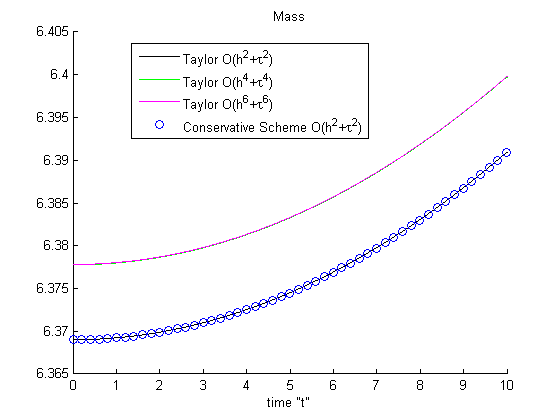
\includegraphics[width=\linewidth]{figures/Mass_bt3_c045_h005_Taylor_Conservative.png}
	\end{minipage}	
	\begin{minipage}[b]{0.4\linewidth}
		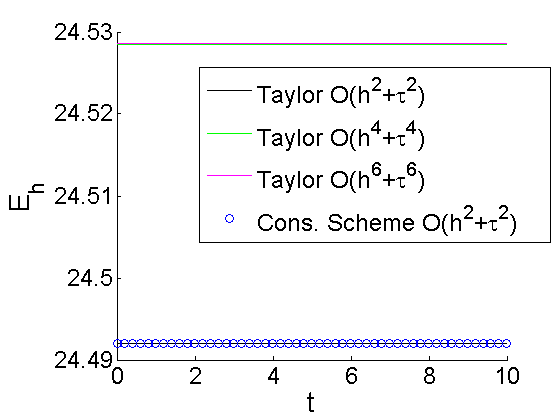
\includegraphics[width=\linewidth]{figures/Energy_bt3_c045_h005_Taylor_Conservative.png}	
	\end{minipage}
\caption{The Mass (left) and Energy (right) of the solution for Test 1, $O(|h|^2 + \tau^2)$ and $T=10$.}
\label{Test1En}
\end{figure}

The Mass increases slightly over the time interval but the gain is neglectable compared to the initial value. For Test 1 the increase with respect to the initial Mass is $0.33\%$ and for Test 2 is $1.8\%$.

\begin{figure}[ht]\vspace{0.2cm}
	\begin{minipage}[b]{0.4\linewidth}
		 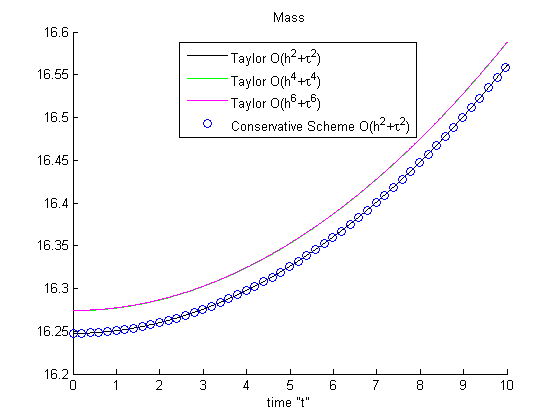
\includegraphics[width=\linewidth]{figures/Mass_bt1_c090_h010_Taylor_Conservative.png}
	\end{minipage}	
	\begin{minipage}[b]{0.4\linewidth}
		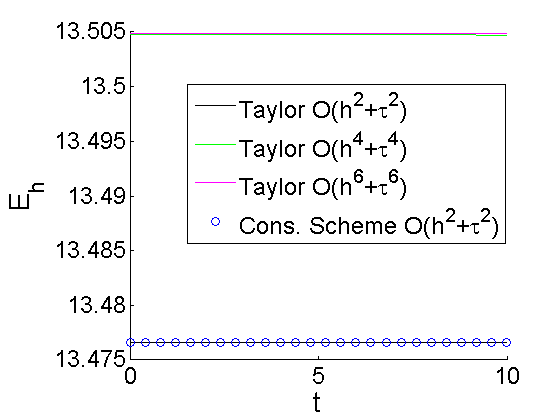
\includegraphics[width=\linewidth]{figures/Energy_bt1_c090_h010_Taylor_Conservative.png}
		
	\end{minipage}
\caption{The Mass (left) and Energy (right) of the solution for Test 2, $O(|h|^2 + \tau^2)$ and $T=10$.}
\label{Test2En}
\end{figure}

For the Taylor Method, the discrete Mass and Energy in Figure \ref{Test1En} and \ref{Test2En} are calculated with three different approximations, namely, trapezoidal formula \rf{quadr2} with $O(h^2)$, Simpson's Rule \rf{quadr4} with $O(h^4)$ and Boole's Rule \rf{quadr6-2D} with $O(h^6)$. It is observed that increasing the order of approximation does not affect the gain for the Mass. It is also confirmed that decreasing the step size $h$ produces similar result, i.e. the graph is slightly shifted upwards or downwards. In the next computations, in order to validate the proper behaviour of the Mass, only the size of the domain is changed whereas the approximation order and discrete steps are fixed.
%----------------------------------------------------------------------------------------------------------------------------------------------
\iffalse
\begin{figure}[ht]\vspace{0.4cm}
	\begin{minipage}[b]{0.33\linewidth}
		 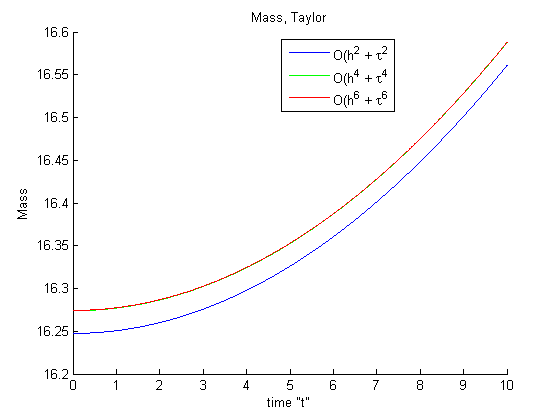
\includegraphics[width=\linewidth]{figures/Mass_bt1_c090_h010_x3O.png}
	\end{minipage}	
	\begin{minipage}[b]{0.33\linewidth}
		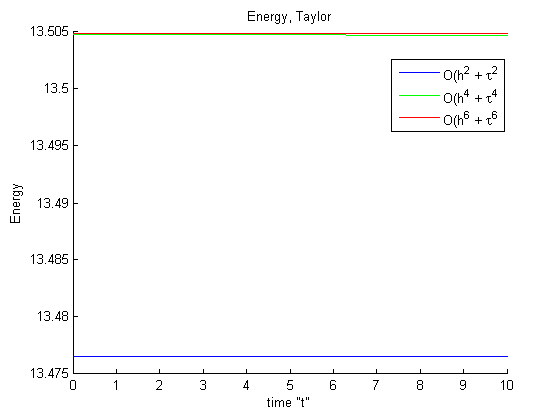
\includegraphics[width=\linewidth]{figures/Energy_bt1_c090_h010_x3O.png}
		
	\end{minipage}
\caption{The Mass (left) and Energy (right) of the Taylor solution for Test 1, $O(|h|^2 + \tau^2)$, $O(|h|^4 + \tau^4)$, $O(|h|^6 + \tau^6)$ and $T=10$.}
\label{Test1TEn}
\end{figure}
\begin{figure}[ht]\vspace{0.4cm}
	\begin{minipage}[b]{0.33\linewidth}
		 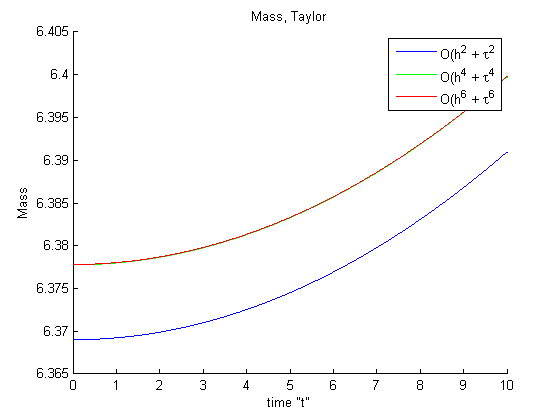
\includegraphics[width=\linewidth]{figures/Mass_bt3_c045_h005_x3O.png}
	\end{minipage}	
	\begin{minipage}[b]{0.33\linewidth}
		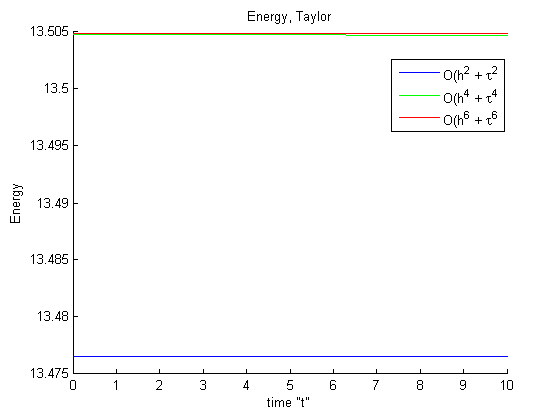
\includegraphics[width=\linewidth]{figures/Energy_bt1_c090_h010_x3O.png}
		
	\end{minipage}
\caption{The Mass (left) and Energy (right) of the Taylor solution for Test 2, $O(|h|^2 + \tau^2)$, $O(|h|^4 + \tau^4)$, $O(|h|^6 + \tau^6)$ and $T=10$.}
\label{Test2TEn}
\end{figure}
\fi
%----------------------------------------------------------------------------------------------------------------------------------------------
If $D$ denotes the discrete Mass, then the percentage gain for the Mass is defined by $100 \times |D(t=0) - D(t=T)|/D(t=0)$. On Figure \ref{Test1_2Mass} one could see that by increasing the size of the domain $\Omega_h$ the gain for the Mass decreases. Taylor method with sixth approximation order and largest step sizes is applied to create the graphs. On the left panel three different domains of size $[-30, 30] \times [-27, 27]$, $[-60, 60] \times [-54, 54]$ and $[-120, 120] \times [-108, 108]$ are used. Furthermore, the used parameter set is $\beta =  3$, $c = 0.45$ (Test 1) and $h=0.2$. The percentage gain for the Mass when increasing the domain is $0.33\%$, $0.11\%$ and $0.06\%$. Analogously, on the right panel, the domains are $[-128, 128] \times [-58, 58]$, $[-256, 256] \times [-116, 116]$ and $[-512, 512] \times [-232, 232]$. The parameter set is $\beta =  1$, $c = 0.9$ (Test 2) and $h=0.4$. Here, the percentage gain for the Mass when increasing the domain is $1.80\%$, $0.70\%$ and $0.18\%$.
\begin{figure}[ht]\vspace{0.2cm}
	\begin{minipage}[b]{0.4\linewidth}
		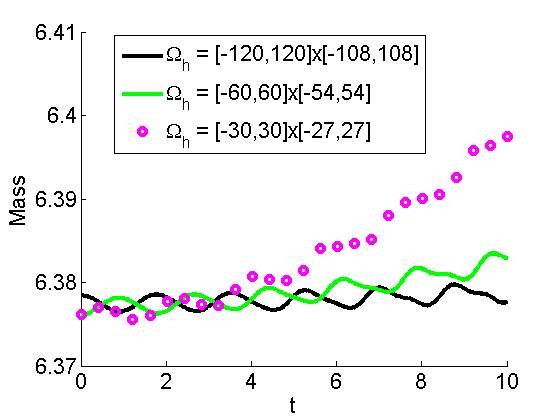
\includegraphics[width=\linewidth]{figures/MassTaylor_120_60_30_ZB1_bt3_c045_h020_O(h^6).png}
	\end{minipage}	
	\begin{minipage}[b]{0.4\linewidth}
		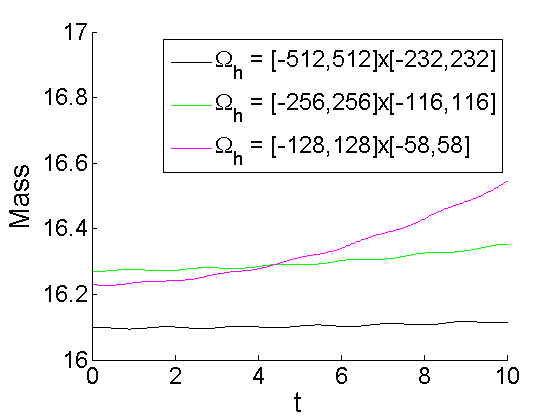
\includegraphics[width=\linewidth]{figures/MassTaylor_512_256_128_ZB1_bt1_c090_h040_O(h^6).png}
		
	\end{minipage}
\caption{The Mass of the Taylor solution for approximation $O(|h|^6 + \tau^6)$ and $T=10$ over three nested domains. Left panel is for $\beta =  3$, $c = 0.45$ and right panel is for $\beta =  1$, $c = 0.9$.}
\label{Test1_2Mass}
\end{figure}

\subsection{Numerical Results for the shape and maximum of the solution}

The following paragraph discusses the shape of the solution obtained by the Conservative FDS and Taylor method. The set up for the calculations is described in Table \ref{tableP} when $p=2$, i.e. both Test 1 and Test 2 are done on three nested meshes. For each Test and mesh both solution techniques are applied with second approximation order. Let us denote with $uC$ and $uT$ the solutions obtained by the Conservative scheme \rf{consFDS} and the TS expansion \rf{TSe}. Figures \ref{Test1_Diff} and \ref{Test2_Diff} show the solution difference for Test 1 and Test 2 respectively. The pictures cover only the center of the domain $\Omega_h$ where the values of the difference are higher. This is one nineth of all mesh points.
\begin{figure}[ht]\vspace{0.4cm}
	\begin{minipage}[b]{0.32\linewidth}
		 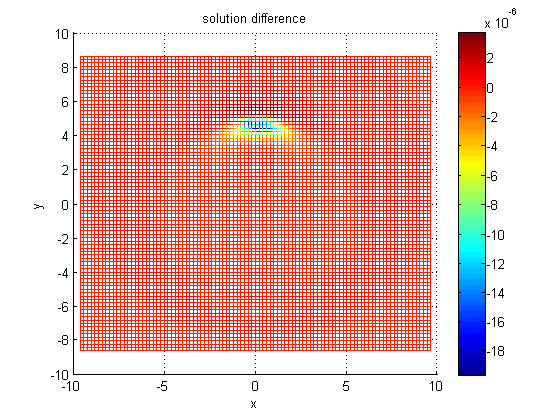
\includegraphics[width=\linewidth]{figures/compare_30_bt3_c045_h020.png}
	\end{minipage}	
	\begin{minipage}[b]{0.32\linewidth}
		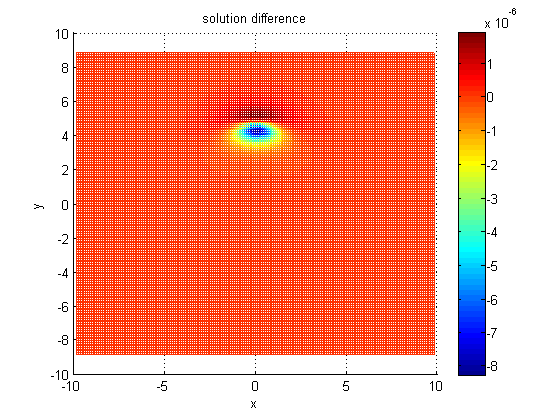
\includegraphics[width=\linewidth]{figures/compare_30_bt3_c045_h010.png}
	\end{minipage}	
	\begin{minipage}[b]{0.32\linewidth}		
		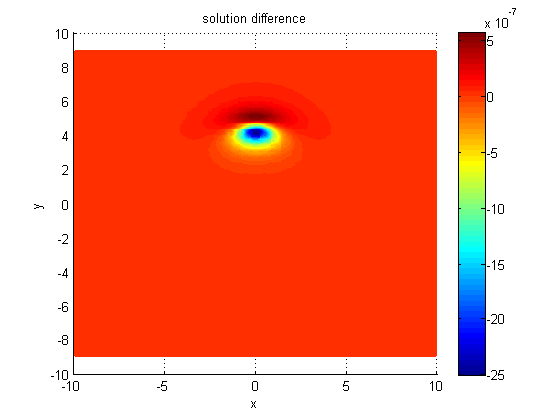
\includegraphics[width=\linewidth]{figures/compare_30_bt3_c045_h005.png}
	\end{minipage}
\caption{Difference $uC - uT$ between solutions from Conservative Scheme and TS approach at time $t=10$, $O(|h|^2 + \tau^2)$ for Test 1. From Left to right $h=0.2, 0.1, 0.05$.}
\label{Test1_Diff}
\end{figure}

\begin{figure}[ht]\vspace{0.4cm}
	\begin{minipage}[b]{0.32\linewidth}
		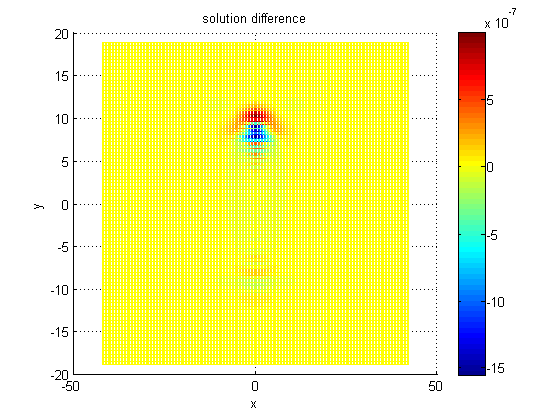
\includegraphics[width=\linewidth]{figures/compare_128_bt1_c09_h040.png}
	\end{minipage}	
	\begin{minipage}[b]{0.32\linewidth}
		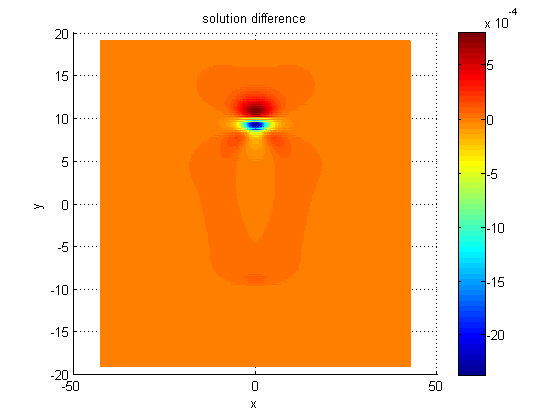
\includegraphics[width=\linewidth]{figures/compare_128_bt1_c09_h020.png}
	\end{minipage}	
	\begin{minipage}[b]{0.32\linewidth}
		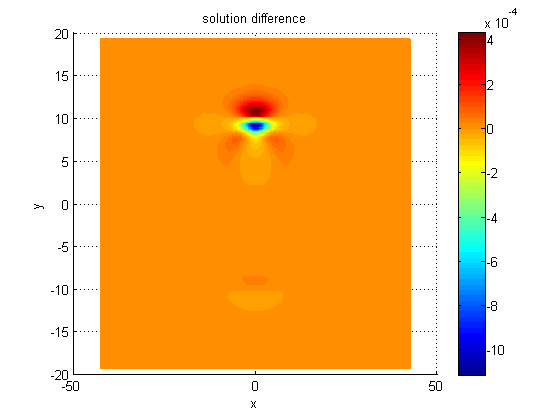
\includegraphics[width=\linewidth]{figures/compare_128_bt1_c09_h010.png}
	\end{minipage}
\caption{Difference $uC - uT$ between solutions from Conservative Scheme and TS approach at time $t=10$, $O(|h|^2 + \tau^2)$ for Test 2. From Left to right $h=0.4, 0.2, 0.1$.}
\label{Test2_Diff}
\end{figure}

\begin{figure}[ht]\vspace{0.2cm}
\centering
	\begin{minipage}[b]{0.30\linewidth}
		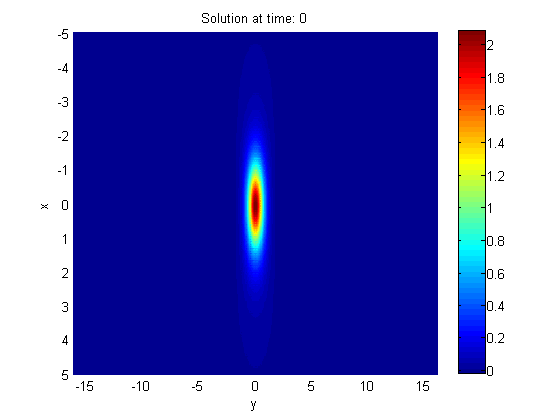
\includegraphics[width=\linewidth]{figures/solution_30x45_bt3_c045_T0.png}
	\end{minipage}	
	\begin{minipage}[b]{0.30\linewidth}
		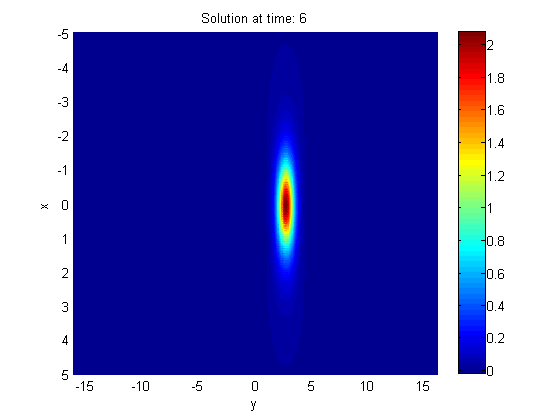
\includegraphics[width=\linewidth]{figures/solution_30x45_bt3_c045_T6.png}
	\end{minipage}	
	\begin{minipage}[b]{0.30\linewidth}
		 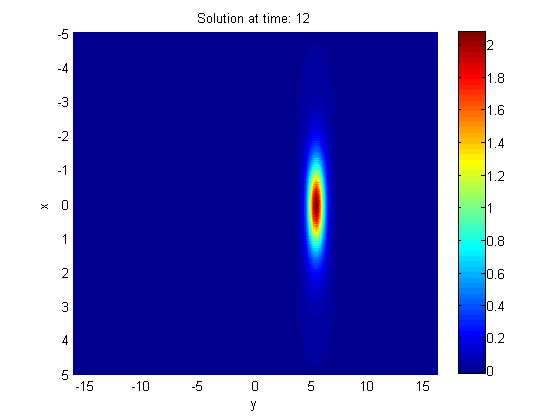
\includegraphics[width=\linewidth]{figures/solution_30x45_bt3_c045_T12.png}
	\end{minipage}
	\begin{minipage}[b]{0.30\linewidth}
		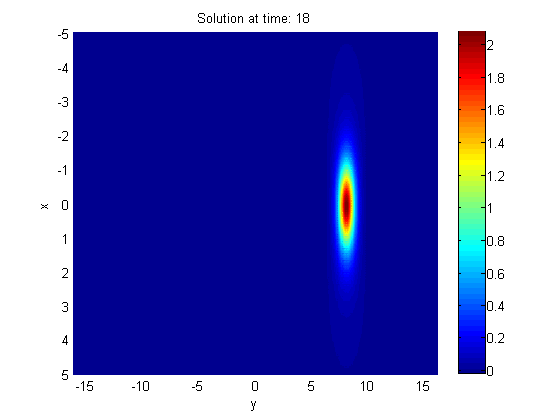
\includegraphics[width=\linewidth]{figures/solution_30x45_bt3_c045_T18.png}
	\end{minipage}	
	\begin{minipage}[b]{0.30\linewidth}
		 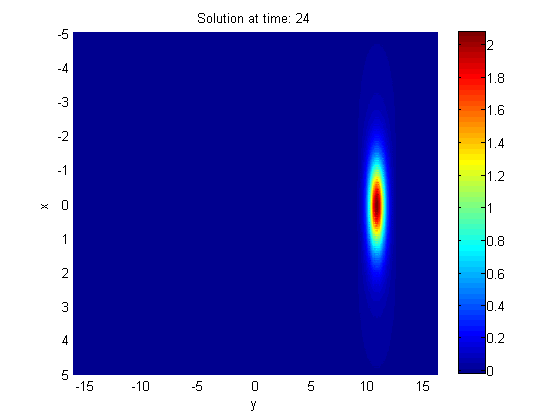
\includegraphics[width=\linewidth]{figures/solution_30x45_bt3_c045_T24.png}
	\end{minipage}
	\begin{minipage}[b]{0.30\linewidth}
		 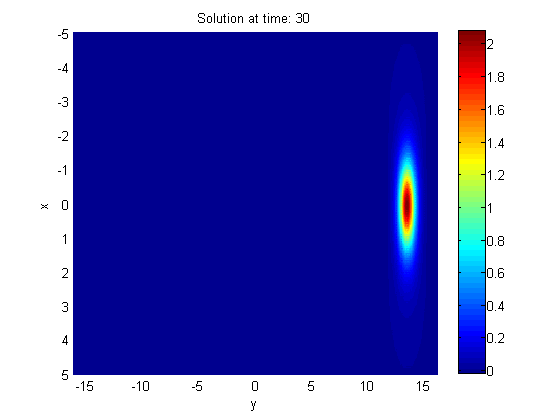
\includegraphics[width=\linewidth]{figures/solution_30x45_bt3_c045_T30.png}
	\end{minipage}
\caption{Numerical solution of single wave for $\beta=3$ and $c = 0.45$ at times $t=0,6,12,18,24,30$.}
\label{Wave1}
\end{figure}

\begin{figure}[ht]\vspace{0.2cm}
\centering
	\begin{minipage}[b]{0.30\linewidth}
		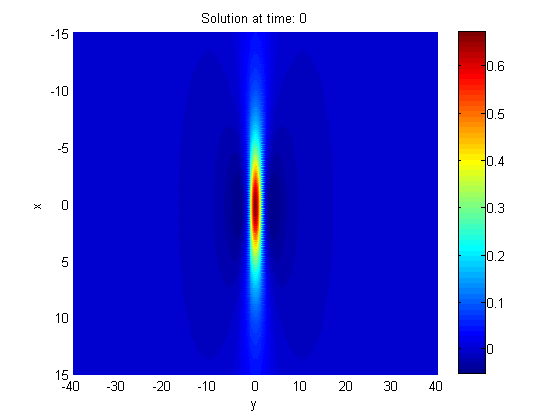
\includegraphics[width=\linewidth]{figures/solution_128x90_bt1_c090_T0.png}
	\end{minipage}	
	\begin{minipage}[b]{0.30\linewidth}
		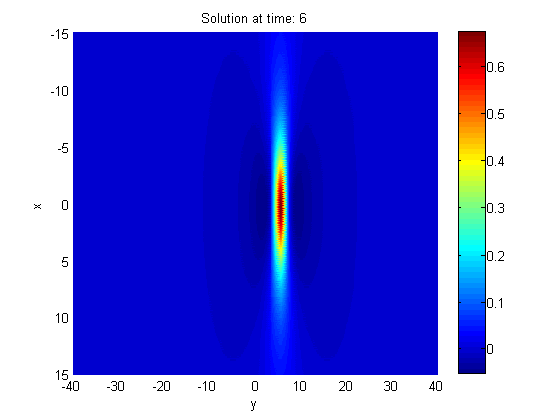
\includegraphics[width=\linewidth]{figures/solution_128x90_bt1_c090_T6.png}
	\end{minipage}	
	\begin{minipage}[b]{0.30\linewidth}
		 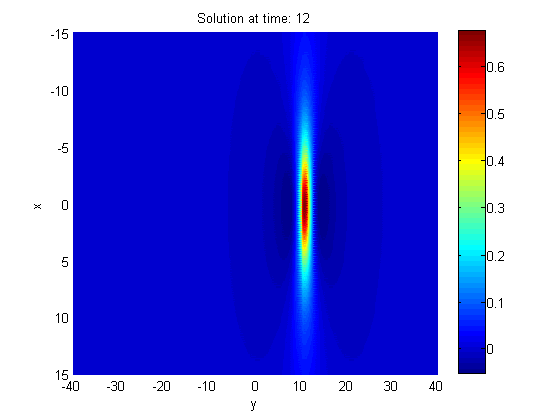
\includegraphics[width=\linewidth]{figures/solution_128x90_bt1_c090_T12.png}
	\end{minipage}
	\begin{minipage}[b]{0.30\linewidth}
		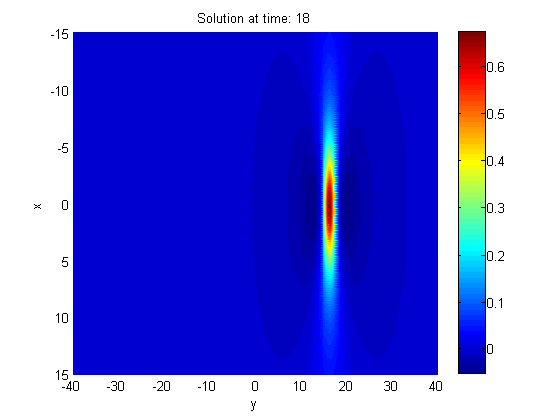
\includegraphics[width=\linewidth]{figures/solution_128x90_bt1_c090_T18.png}
	\end{minipage}	
	\begin{minipage}[b]{0.30\linewidth}
		 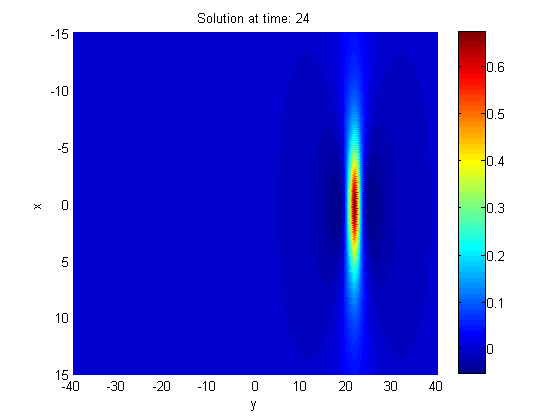
\includegraphics[width=\linewidth]{figures/solution_128x90_bt1_c090_T24.png}
	\end{minipage}
	\begin{minipage}[b]{0.30\linewidth}
		 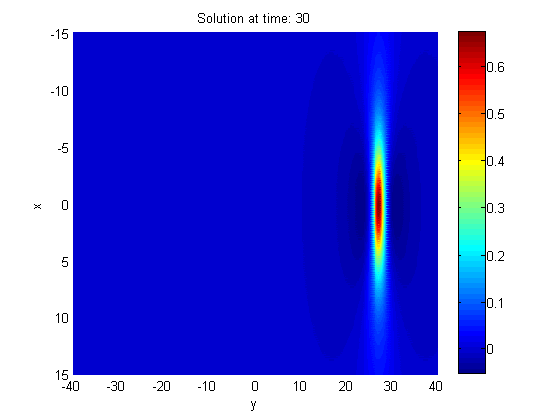
\includegraphics[width=\linewidth]{figures/solution_128x90_bt1_c090_T30.png}
	\end{minipage}
\caption{Numerical solution of single wave for $\beta=1$ and $c = 0.9$ at times $t=0,6,12,18,24,30$.}
\label{Wave2}
\end{figure}
The figures are for visual representation. On the contrary, Table \ref{tableF} shows the difference $||uC - uT||_\kappa$ using $L_2$ and infinity norms. The last column of the Table is for the infinity norm of the solution $||uC||_{L_\infty}$ (which is the wave maximum) measured by the Conservative FDS. It is observed that decreasing the step sizes $h$ and $\tau$ results in a smaller difference.  Furthermore the percentage difference when using the infinity norm
$$\frac{ ||uC - uT||_{L_\infty}} { ||uC||_{L_\infty} } \times 100$$
varies in the inteval $[0.0001\%, 0.69\%]$ for all rows in the table. Analogous results are obtained for the percentage difference when using the $L_2$ norm and thus are omitted. The difference between the wave shapes obtained by Conservative FDS and the Taylor Series approach with Method of lines is negligible. It is expected that $||uC - uT||_\kappa$ goes to zero when $h$ and $\tau$ are infinitely small.

%F
\begin{table}[ht]
\centering
\small
		\begin{tabular}{||c|l|l|l|l||}
			\hline
			\hline
      FDS        &$h$, $\tau$  &   $||uC - uT||$  in $L_2$     &  $||uC - uT||$ in $L_\infty$ & $||uC||$ in $L_\infty$ \\
   			\hline 
					\hline 
  $\beta=3$                   &0.2, 0.001         &  1.749e-05      &  1.965e-05  & 1.315448     \\
   c=0.45                        &0.1, 0.0005        &  8.109e-06       & 8.274e-06 &  1.862688     \\
     $O(h^2 + \tau^ 2)$ &0.05, 0.00025     & 2.460e-06         &2.502e-06  &   2.013184   \\
			\hline 
			\hline 
       $\beta=1$          &0.4, 0.002        & 0.009981     & 0.004560 & 0.656747   \\
                  c=0.9      &0.2, 0.001        & 0.005047      & 0.002373  & 0.673901   \\
  $O(h^2+ \tau^2)$ &0.1, 0.0005         & 0.002521      &0.001117 & 0.672231   \\
			\hline
	   \hline
			\hline 
		\end{tabular}
		\caption{Difference $uC - uT$ between solutions from Conservative Scheme and TS approach at time $t=10$ with $O(|h|^2 + \tau^2)$ approximation errors. Differences are measured in $L_2$ and $L_\infty$ norms.}
\label{tableF}
\end{table}

The following paragraph discusses the preservation of the solution's shape over the time interval $[0, 10]$. The set up for the calculations is described in Table \ref{tableP} when using the Taylor method, i.e. $p=2, 4, 6$ and for each approximation order, three nested meshes are used. For more details refer to Table \ref{tableG}. Here, the first column is for the Test case. The second describes the spatial step size $h$. The third and fourth columns present the solution difference at times $t=0$ and $t=10$ in $L_2$ and $L_\infty$ norms. The wave travels a distance which is equal to the speed $c$ multiplied by the end time $T$. Thus, the maximum of the solution at time $t=10$ is located on $(0, 10 c) \in \Omega$. The maximum at time $t=0$ is located on $(0, 0) \in \Omega$. Unfortunately, for Test 1, $h=0.2$ and Test 2, $h=0.4$ the maximum for $t=10$ is not inside the mesh. Further calculations are done to shift the wave along the $y$ axis so that the maximum fall under the closest available meshpoint. For Test 1 ($c=0.45$) the wave travels additional distance of 0.1 for time 2/9 which shifts the maximum to a position of $(0, 4.6) \in \Omega_h$. For Test 2 ($c=0.9$) the wave travels additional distance of 0.2 for time 2/9 which shifts the maximum to a position of $(0, 9.2) \in \Omega_h$. The subtraction of two solutions $u^{(0)} - u^{(N_t)}$ results in a matrix with the following coefficients:
$$ \delta_{i,j} = u_{i,j}^{(0)} - u_{i,j+cT/h}^{(N_t)},$$
where $0 < i < N_x$ and $0 < j < N_y - cT/h$. 

%G
\begin{table}[ht]
\centering
\small
		\begin{tabular}{||c|l|l|l||}
			\hline
			\hline
      FDS        & $h$, $\tau$  & $||u^{(0)} - u^{(N_t)}||$ in $L_2$  & $||u^{(0)} - u^{(N_t)}||$ in $L_\infty$   \\
   		\hline 
			\hline
  $\beta=3$                &0.2, 0.001\footnote{Position of maximum is further adjusted to fit inside $\Omega_h$.}            & 1.494351 & 1.533173    \\
   c=0.45                     &0.1, 0.0005          & 0.466991 & 0.484011       \\
     $O(h^2 + \tau^ 2)$ &0.05, 0.00025   & 0.127641 & 0.132504      \\
			\hline 
  $\beta=3$               &0.2, 0.02 $^{\text{a}}$      &0.220560 & 0.230486       \\
   c=0.45                    &0.1, 0.01      &0.013762 & 0.014391        \\
     $O(h^4+ \tau^4)$ &0.05, 0.005&0.000877 & 0.000917         \\
			\hline 
  $\beta=3$               &0.2, 0.02 $^{\text{a}}$       &  0.035965 & 0.038039        \\
     c=0.45                 &0.1, 0.01        &0.000600 & 0.000633       \\
     $O(h^6+ \tau^6)$ &0.05, 0.005 &0.000010 & 0.000010          \\
	   \hline
			\hline 
       $\beta=1$       &0.4, 0.002 $^{\text{a}}$       & 0.244208 & 0.103833 \\
                  c=0.9    &0.2, 0.001       &  0.057175 & 0.026919  \\
  $O(h^2+ \tau^2)$ &0.1, 0.0005   & 0.013938 & 0.006622  \\
			\hline
      $\beta=1$               &0.4, 0.04 $^{\text{a}}$    &0.028546 & 0.012203 \\
       c=0.9                     &0.2, 0.02     & 0.001757 & 0.000958     \\
       $O(h^4+ \tau^4)$ &0.1, 0.01   & 0.000112 & 0.000061   \\
    \hline
  $\beta=1$                  &0.4, 0.04 $^{\text{a}}$   &0.006415 & 0.002792  \\
      c=0.9                    &0.2, 0.02   &0.000112 & 0.000065     \\
     $O(h^6+ \tau^6)$ &0.1, 0.01 & 0.000002 & 0.000001         \\
	   \hline
			\hline 
		\end{tabular}
		\caption{Difference $||u^{(0)} - u^{(N_t)}||_\kappa$ in $L_2$ and $L_\infty$ norms between solutions at time $t=0$ and $t=10$. TS approach is used for all measurements in the table.}
\label{tableG}
\end{table}

Table \ref{tableG} shows that if the step size $h$ (and $\tau$ respectively) decreases, then the difference also decreases. Furthermore, the shape of the wave is preserved better while the approximation order $p$ increases. Thus, it is expected that $||u^{(0)} - u^{(N_t)}||_\kappa$ goes to zero when $h$ and $\tau$ are infinitely small. 

\begin{figure}[H]\vspace{0.2cm}
	\centering
	\begin{minipage}[b]{0.40\linewidth}
		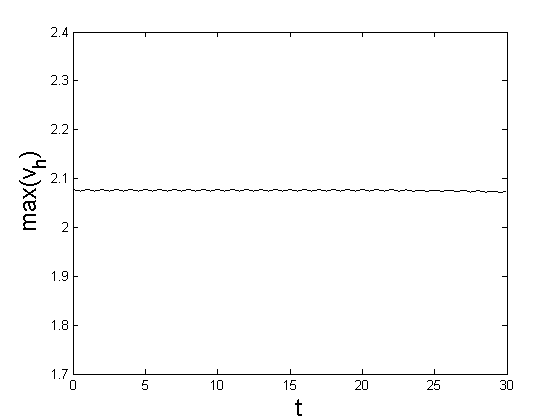
\includegraphics[width=\linewidth]{figures/maximum_30_T30_bt3_c045_h005.png}
	\end{minipage}	
	\begin{minipage}[b]{0.40\linewidth}
		 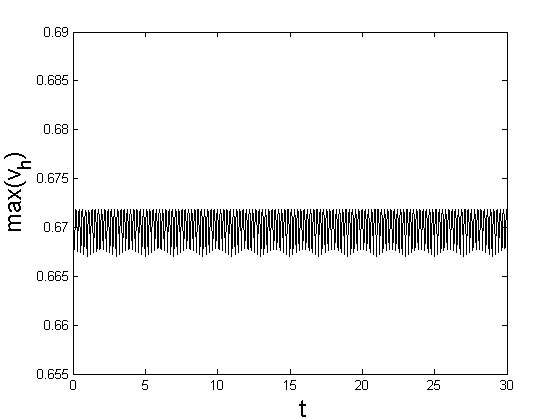
\includegraphics[width=\linewidth]{figures/maximum_30_T30_bt1_c090_h020.png}
	\end{minipage}
\caption{Evolution of the maximum over a larger time interval $[0, 30]$ for Test 1 (left panel) and Test 2 (right panel).}
\label{Maximum}
\end{figure}

The following paragraph discusses the maximum of the solution over a larger time interval $[0, 30]$. The set up for the two calculations is described in Table \ref{tableP} where 
$p=6$, $T=30$ and Taylor method is applied with $h=0.05$ and $\tau = 0.001$ for Test 1 and $h=0.2$ and $\tau=0.02$ for Test 2. Also the size of the computational box $\Omega_h$ is extended appropriately along the $y$ axis to compensate for the wave shift. Figure \ref{Maximum} shows that the maximum is stable for both tests over a larger time interval $[0, 30]$. For each iteration step, the exact position of the maximum is not always located on a mesh point in $\Omega_h$. This produces a jagged graph which is well expressed on the right panel and also present on the left panel in Figure \ref{Maximum}. Solution shapes are shown in Figures \ref{Wave1} and \ref{Wave2}.

\section{Conclusion}
The 2D BPE is solved using Taylor method with high approximation orders $O(|h|^p + \tau^p)$, $p=2, 4, 6$. The results are compared with the Conservative FDS for $O(|h|^2 + \tau^2)$. Solutions from both methods are qualitatively and quantitatively very similar. Runge's Rule show that the discrete solution and Energy converge for all numerical calculations described in Table \ref{tableP}. The Mass and Energy of the Taylor method are saved with high accuracy over the time interval $[0, 10]$. The discrete Energy is a constant function of the time variable. It is hard to measure the Mass which is defined as an infinite integral of the solution. Computational tests show that the discrete Mass slightly increases as the wave moves. Nevertheless, it is obtained that the gain for the discrete Mass diminishes when the domain $\Omega_h$ grows. The numerical solutions for wave speeds near the upper limit $c_{max} = min(1, \sqrt{\beta_2/\beta_1})$ are stable in form over the time interval $[0, 10]$. It is seen that the change in the shape decreases when the step sizes $h$ and $\tau$ contract or the approximation order $p$ increases. The behaviour of the maximum over a long period of time $[0, 30]$ is preserved with small errors.

%\begin{acknowledgments}
%The work of the second author has been partially supported by the Bulgarian Science Fund under grant K$\Pi$-06-H22/2.
%\end{acknowledgments}

%\nocite{*}
%\bibliography{aipsamp}% Produces the bibliography via BibTeX.

\begin{thebibliography}{99} \normalsize

\bibitem{ref16} Angelow, K., Kolkovksa, N., Numercal Study of Traveling Wave Solutions to 2D Boussinesq Equation, {\it Serdica J. Computing}, \textbf{13} (2019), 1-16.

\bibitem{ref0} Boussinesq, J.V., Theorie des ondes et des remous qui se propagent le long d'un canal rectangulaire horizontal, en communiquant au liquide contenu dans ce canal des vitesses sensiblement pareilles de la surface au fond.  {\it Journal de Mathematiques Pures et Appliquees}, \textbf{17} (1872), 55-108.

\bibitem{ref21} Chertok, A., Christov, C.I., Kurganov, A., Central-Upwind Schemes for the Boussinesq Paradigm Equations,
{\it Computational Science and High Performance Computing IV, Notes Numer. Fluid Mech.}, \textbf{113} (2011), 267-281.

\bibitem{ref13}  Christou M. , Christov C.I.,
Galerkin spectral method for the 2D solitary waves of Boussinesq paradigm equation,
In: {\it Applications of Mathematics in Technical and Natural Sciences, Sozopol (Bulgaria)},
\emph{AIP Conference Proceedings}, \textbf{1186}, Issue 1 (2009), 217-225.

\bibitem{ref14}  Christou M. , Christov C.I.,
Fourier Galerkin method for 2D solitons of Boussinesq equation,
{\it Mathematics and Computers in Simulation} \textbf{74} (2007), 82-92.

\bibitem{ref1} Christov, C.I., An energy-consistent dispersive shallow-water model,  {\it Wave Motion}, \textbf{34} (2001), 161-174.

\bibitem{ref15} Christov, C.I., Choudhury, J., Perturbation solution for the 2D Boussinesq equation, {\it Mech. Res. Commun.}, \textbf{38} (2011), 274-281.

\bibitem{ref4} Christov, I., Christov, C.I., Physical dynamics of quasi-particles in nonlinear wave equations,
{\it Physics Letters A}, \textbf{372}, Issue 4 (2008),  841-848.

\bibitem{ref20} Christov, C.I., Kolkovska, N., Vasileva, D., On the Numerical Simulation of Un-
steady Solutions for the 2D Boussinesq Paragigm Equation,
{\it In: I. Dimov, S. Dimova, N. Kolkovska (Eds.), Numerical Methods and Applications 2010},
\emph{Conference Proceedings}, \textbf{6046} (2010), 386–394.

\bibitem{ref23} Dimova M., Vasileva D., Comparison of Two Numerical Approaches to Boussinesq Paradigm Equation, 
{\it Lect. Notes Comput. Sci.}, \textbf{8236} (2013), 255-262.

\bibitem{forn}
Fornberg, B., Generation of Finite Difference Formulas on Arbitrarily Spaced Grids, 
Math. Comput., 51(1988),  699 -- 706.

\bibitem{ref25} Kolkovska N., Two families of finite difference schemes for multidimensional Boussinesq paradigm equation, In:
{\it Applications of Mathematics in Technical and Natural Sciences,  Sozopol (Bulgaria)},
\emph{AIP Conference Proceedings}, \textbf{1301} (2010), 395.

\bibitem{ref22} Kolkovska, N., Angelow K., A Multicomponent Alternating Direction Method for Numerical Solving of Boussinesq Paradigm Equation,
In: {\it  I. Dimov, I., Farago, I., Vulkov, L. (eds.) NAA 2012},
\emph{Conference Proceedings}, \textbf{8236} (2013), 371–378.

\bibitem{samarski} Samarskii, A., The Theory of Difference Schemes, Marcel Dekker Inc., New York, 2001.
%
\end{thebibliography}
\end{document}
%
% ****** End of file aipsamp.tex ******